\documentclass[11pt,oneside,a4paper]{article}
\setlength{\emergencystretch}{3em}

% ==============================
% ENCODING
% ==============================
\usepackage[utf8]{inputenc}
\usepackage[T1]{fontenc}

% ==============================
% PAGE LAYOUT
% ==============================
\usepackage{geometry}
\geometry{
    a4paper,
    top=2.5cm,
    bottom=2.5cm,
    left=3cm,
    right=3cm
}

\usepackage{setspace}
\onehalfspacing

% ==============================
% FONTS
% ==============================
% \usepackage[scaled]{helvet}
% \renewcommand{\familydefault}{\sfdefault}
\usepackage{lmodern}
% ==============================
% MATH & SYMBOLS
% ==============================
\usepackage{amsmath, amsthm, amsfonts}
\usepackage{siunitx}

% ==============================
% TABLES & FIGURES
% ==============================
\usepackage{graphicx}
\usepackage{subfig}
\usepackage{array}
\usepackage{makecell}
\usepackage{multirow}
\usepackage{adjustbox}
\usepackage{threeparttable}
\usepackage{tablefootnote}
\usepackage{booktabs} 

% ==============================
% CHAPTER FORMATTING
% ==============================
\usepackage{titlesec}

\titleformat{\chapter}
{\normalfont\huge\bfseries}
{\thechapter.}
{20pt}
{\huge\bfseries}

% ==============================
% NUMBERING
% ==============================
\usepackage{chngcntr}
\counterwithin{figure}{chapter}
\counterwithin{table}{chapter}

% ==============================
% BIBLIOGRAPHY
% ==============================
\usepackage{csquotes}

\usepackage[
backend=biber,
style=ieee
]{biblatex}

\addbibresource{References.bib}

% ==============================
% GLOSSARY & ACRONYMS
% ==============================
\usepackage[acronym,toc]{glossaries-extra}

% ==============================
% DIAGRAMS
% ==============================
\usepackage{tikz}

% ==============================
% COLORS
% ==============================
\usepackage{xcolor}

\definecolor{CPUTBlue}{HTML}{005696}
\definecolor{CPUTRed}{HTML}{ED1C24}

% ==============================
% PROFESSIONAL HEADERS
% ==============================

\usepackage{fancyhdr}

\setlength{\headheight}{18pt}

\pagestyle{fancy}
\fancyhf{}

\fancyhead[L]{\small SDN260S SOFTWARE DESIGN 2}
\fancyhead[R]{\small\nouppercase{\leftmark}}

\fancyfoot[C]{\thepage}

\renewcommand{\headrulewidth}{0.4pt}
\renewcommand{\footrulewidth}{0pt}

% ==============================
% PDF / LINKS
% ==============================
\usepackage{hyperref}

\hypersetup{
colorlinks=true,
linkcolor=black,
citecolor=black,
urlcolor=blue,
pdftitle={SOFTWARE DESIGN 2 Group 3 Report 2026}
}

% ==============================
% QUALITY IMPROVEMENTS
% ==============================
\usepackage{microtype}

% ==============================
% MISC
% ==============================
\usepackage{pdfpages}
\usepackage{lipsum}

% --- CPUT REPORT INFORMATION ---
\newcommand*{\getUniversity}{Cape Peninsula University of Technology}
\newcommand*{\getFaculty}{Faculty of Engineering and the Built Environment}
\newcommand*{\getDepartment}{Department of Electrical, Electronic, and Computer Engineering}

\newcommand*{\getTitle}{%
\fontsize{16pt}{18pt}\selectfont\bfseries
Development and Implementation of a Marks Administration System for the Cape Peninsula University of Technology\\[0.6em]
\large System Design Document\\[0.4em]
}

\newcommand*{\getAuthor}{Group 3}
\newcommand*{\getDoctype}{Group project report submitted in partial fulfilment of the requirements for the degree}
\newcommand*{\getDegree}{Bachelor of Engineering Technology in Computer Engineering}
\newcommand*{\getSupervisor}{Mr. Stephen Ekwe}
\newcommand*{\getCourseCode}{SDN260S - SOFTWARE DESIGN 2}
\newcommand*{\getCampus}{Bellville Campus}
\newcommand*{\getSubmissionDate}{November 2026}
\newcommand*{\getCopyright}{
The report may not be published either in part
(in scholarly, scientific or technical journals), or as a whole
(as a monograph), unless permission has been obtained from the University.
}

% --- Project links and graduate attribute titles (fill in / confirm) ---
\newcommand*{\githubLink}{\url{https://github.com/anh-duynguyen/SDN260S_SOFTWARE_DESIGN_2_Group_3_Project}}
\newcommand*{\gaTwoName}{GA2: Application of Scientific and Engineering Knowledge}
\newcommand*{\gaSevenName}{GA7: Impact of Engineering Activity}

\begin{document}

% -------------------------------
% FRONT MATTER (not counted in the 10-page limit)
% -------------------------------
\pagenumbering{roman}
\begin{titlepage}
    \begin{center}

        % --- Header block: logo + institution ---
        \IfFileExists{Images/logo_CPUT.png}{%
            
\includegraphics[height=25mm]{Images/logo_CPUT.png}
        }{%
            \vspace*{25mm}
        }

        \vspace{4mm}
        {\large \scshape Department of Electrical, Electronic and Computer Engineering\par}

        \vfill

        % --- Title block ---
        \rule{0.8\textwidth}{0.4pt}\\[6mm]
        {\huge \bfseries \getTitle \par}
        \vspace{3mm}
        \rule{0.8\textwidth}{0.4pt}

        \vspace{11mm}

        {\Large by}\\[4mm]
        {\Large \bfseries \getAuthor}

        \vfill

        % --- Degree statement ---
        {\large \getDoctype}\\[0.4cm]
        {\large \bfseries \getDegree}\\[0.4cm]
        {\large in the \getFaculty}\\[0.4cm]
        {\large at the \getUniversity}

        \vfill

        % --- Examiner / course info ---
        \begin{tabular}{r l}
            Examiner:    & \getSupervisor \\
            Course Code: & \getCourseCode \\
            % \ifx\getCoSupervisor\empty \else Co-supervisor: & \getCoSupervisor \\ \fi
        \end{tabular}

        \vspace{5mm}

        {\large \getCampus}\\
        {\large \getSubmissionDate}

        \vfill

        % --- Copyright statement ---
        \begin{minipage}{0.8\textwidth}
            \centering
            \footnotesize \getCopyright
        \end{minipage}

    \end{center}
\end{titlepage}
\setcounter{page}{1}
\section*{Declaration of Authorship}
\addcontentsline{toc}{section}{Declaration of Authorship}

We, the undersigned, declare that the contents of this report represent our own unaided work, except where explicitly acknowledged. The report has not previously been submitted for academic examination towards any qualification. Furthermore, it represents our own opinions and not necessarily those of the Cape Peninsula University of Technology.

\vspace{6mm}

% \sigcell{file}{width}{height}: signature image if it exists, otherwise an empty space to sign by hand.
\newcommand{\sigcell}[3]{\parbox[b][#3][b]{6.2cm}{\centering\IfFileExists{Images/#1.png}{\includegraphics[width=#2,height=#3,keepaspectratio]{Images/#1.png}}{\rule{0pt}{#3}}}}
\newcommand{\sigrow}[6]{%
\sigcell{#1}{#5}{#6} & \sigcell{#2}{#5}{#6} \\
\rule{6.2cm}{0.4pt} & \rule{6.2cm}{0.4pt} \\
#3 & #4 \\[4mm]}

\begin{tabular}{@{}p{6.2cm} p{6.2cm}@{}}
\sigrow{signature_anh_duy_nguyen}{signature_carl_lamprecht}{Anh Duy Nguyen, 251163733}{Carl Leonard Lamprecht, 205133681}{4.2cm}{1.5cm}
\sigrow{signature_jaunne_havenga}{signature_Keno_Solomons}{Jaunne Alex Havenga, 240178394}{Keno Solomons, 250151448}{4.2cm}{1.5cm}
\sigrow{signature_gian_koekemoer}{signature_peter_ngesi}{Gian Koekemoer, 250060248}{Peter Hlalubonga Ngesi, 250281228}{4.2cm}{1.5cm}
\sigrow{signature_pedro_weir}{signature_uthmaan_carelse}{Pedro Josh Weir, 250531836}{Uthmaan Carelse, 251419274}{4.2cm}{1.5cm}
\today \\[1mm]
\rule{6.2cm}{0.4pt} \\
\footnotesize Date
\end{tabular}

\clearpage
\section*{AI Declaration}
\addcontentsline{toc}{section}{AI Declaration}

We declare that generative artificial intelligence (AI) tools were used in the preparation of this report as follows:

\begin{itemize}
    \item \textbf{Grammar, spelling, and language refinement} (e.g., rephrasing for clarity and readability).
    \item \textbf{LaTeX formatting assistance} (structure and code improvements).
    \item \textbf{Drafting and structuring of report sections} from the group's source code, earlier check-in reports, word documents (from Alex and Keno) and notes.
\end{itemize}

All AI-generated suggestions were reviewed, edited, and verified by the authors against the source code and test results. The design decisions, implementation and testing described are the work of the authors. This declaration is made in accordance with academic integrity principles and the Cape Peninsula University of Technology guidelines on responsible AI use.

\vspace{6mm}
\begin{tabular}{@{}p{6.2cm} p{6.2cm}@{}}
\sigrow{signature_anh_duy_nguyen}{signature_carl_lamprecht}{Anh Duy Nguyen, 251163733}{Carl Leonard Lamprecht, 205133681}{2.6cm}{0.9cm}
\sigrow{signature_jaunne_havenga}{signature_Keno_Solomons}{Jaunne Alex Havenga, 240178394}{Keno Solomons, 250151448}{2.6cm}{0.9cm}
\sigrow{signature_gian_koekemoer}{signature_peter_ngesi}{Gian Koekemoer, 250060248}{Peter Hlalubonga Ngesi, 250281228}{2.6cm}{0.9cm}
\sigrow{signature_pedro_weir}{signature_uthmaan_carelse}{Pedro Josh Weir, 250531836}{Uthmaan Carelse, 251419274}{2.6cm}{0.9cm}
\end{tabular}

\clearpage
\chapter*{Abstract}

\lipsum

\vspace{5mm}
\textbf{Keywords:} CPUT, Conmputer, Java
\clearpage
\tableofcontents
\clearpage
\listoffigures
\listoftables

% -------------------------------
% MAIN MATTER (10 pages maximum)
% -------------------------------
\clearpage
\pagenumbering{arabic}
\setcounter{page}{1}

\section{Introduction and Problem Statement}

\subsection{The problem}
A lecturer records several assessments for every student in a course, such as a test, a practical and an examination. Each assessment has its own maximum mark and its own weight in the final result. The lecturer must then calculate each student's final mark, notice which students still have outstanding marks, and report class performance to the Head of Department. When this is done by hand in spreadsheets, three weaknesses appear:
\begin{enumerate}
  \item final marks depend on formulas that can be broken, mistyped or weighted incorrectly;
  \item a missing mark is easy to overlook and silently distorts totals and class averages;
  \item nothing separates the people who may change marks from the people who may only view them.
\end{enumerate}
Because marks decide progression, an error in any of these areas has real consequences for students.

\subsection{Objectives and scope}
The Marks Administration System is a Java desktop application that addresses the problems above. Its objectives are to:
\begin{itemize}
  \item capture, update, import and export student marks, with automatic calculation of the weighted final mark and symbol;
  \item flag missing marks and keep them out of class statistics;
  \item produce student reports and class summaries, including rankings and grade distributions;
  \item enforce role-based access for lecturers (edit) and Heads of Department (read-only);
  \item support several courses, each with its own data file.
\end{itemize}
The application is written in plain Java 17 with a Swing interface and no third-party libraries, so persistence uses CSV files rather than a database server. It is a single-user desktop prototype. Password protection was developed on a separate branch and is awaiting review, so it is not part of the delivered feature set. Earlier progress is recorded in the Check-in 1 and Check-in 2 reports, which are not repeated here.

\subsection{Structure of this document}
Sections~\ref{sec:arch} and~\ref{sec:decisions} present the class design and design decisions, Sections~\ref{sec:algos} to~\ref{sec:adv} the algorithms, implementation and advanced features, and Section~\ref{sec:testing} the testing strategy. Sections~\ref{sec:reflect} and~\ref{sec:team} cover the GA2 and GA7 reflections and the team process, and Section~\ref{sec:concl} concludes.

\section{System Architecture and Class Design}\label{sec:arch}

\subsection{Layered architecture}
The system is split into four layers so that each can change without disturbing the others. The \emph{presentation layer} (\texttt{Main}, \texttt{GUI}) only displays information and collects input. The \emph{role layer} (\texttt{User}, \texttt{Lecturer}, \texttt{HeadOfDepartment}) decides what each kind of user may do and returns results as text. The \emph{domain layer} (\texttt{Course}, \texttt{Student}, \texttt{AssessmentComponent}, \texttt{IndividualMarksManager}, \texttt{StudentManager}, \texttt{CollectiveMarksManager}) holds the marks and the calculations. The \emph{persistence layer} (\texttt{Database}) reads and writes CSV files. \texttt{CourseSessionCoordinator} sits between the interface and the rest, tracking which course is active and which data belongs to it.

\subsection{UML Class Diagram}

Figure~\ref{fig:uml} shows the main classes. Attributes and methods are abbreviated; lines without parentheses describe a responsibility rather than an exact member name.

\begin{figure}[htbp]
    \centering
    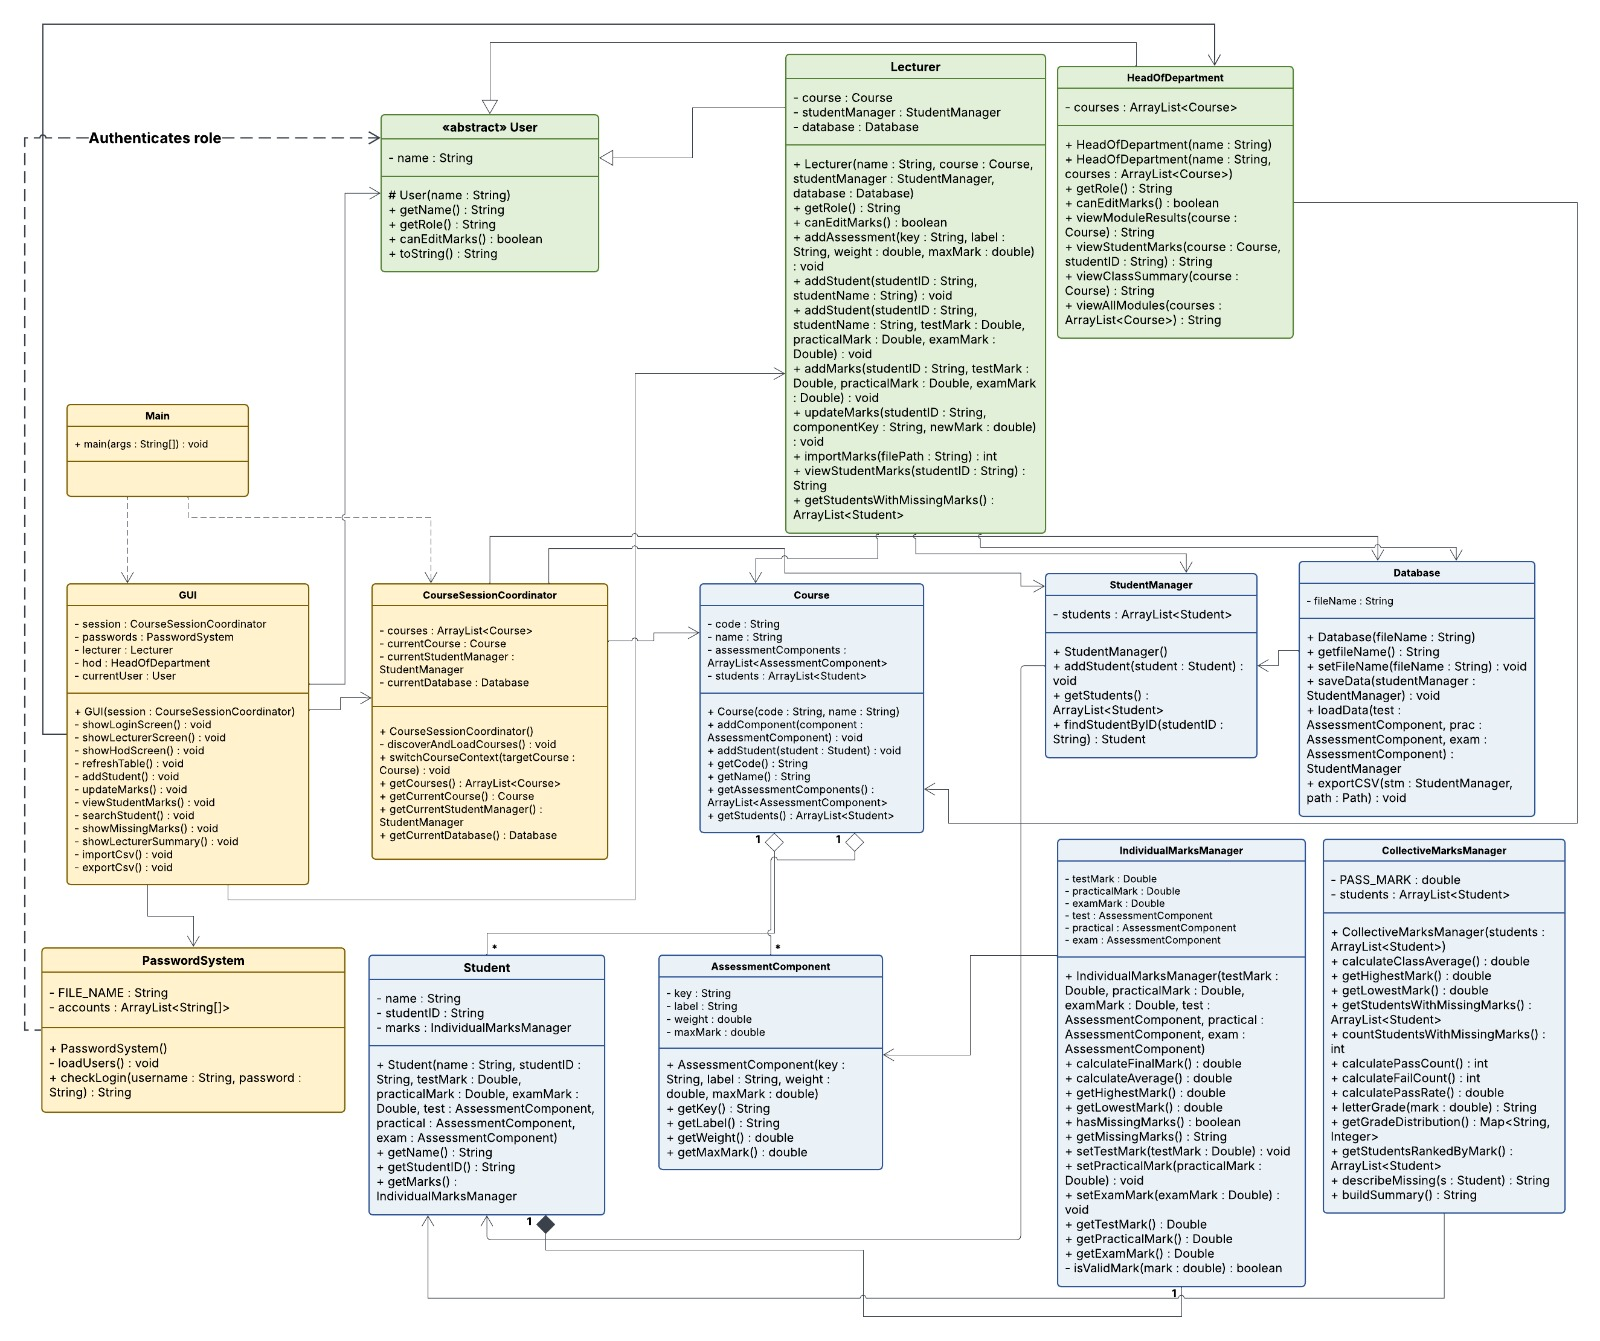
\includegraphics[width=0.9\textwidth]{Images/uml_diagram.jpeg}
    \caption{UML class diagram of the Marks Administration System.}
    \label{fig:uml}
\end{figure}

\subsection{Class responsibilities and relationships}
\begin{table}[htbp]
\centering
\footnotesize
\renewcommand{\arraystretch}{1.05}
\caption{Main classes and their responsibilities.}
\label{tab:classes}
\begin{tabularx}{\textwidth}{@{}l X@{}}
\toprule
\textbf{Class} & \textbf{Responsibility}\\
\midrule
\texttt{GUI} & Login, lecturer table and Head of Department dashboard; turns exceptions into dialogs.\\
\texttt{CourseSessionCoordinator} & Keeps the list of courses, the active course and its \texttt{StudentManager} and \texttt{Database}.\\
\texttt{User} (abstract) & Validates the name and defines the role and mark-editing permission shared by all users.\\
\texttt{Lecturer} & Adds students, captures and updates marks, imports and exports CSV, views reports.\\
\texttt{HeadOfDepartment} & Read-only inspection of course results, class summaries and student marks; manages the course list.\\
\texttt{Course} & Holds a course code and name, its assessment components and its students.\\
\texttt{AssessmentComponent} & Describes one assessment: key, label, weight and maximum mark.\\
\texttt{Student}, \texttt{StudentManager} & A student's identity and marks; the collection of students with lookup by student number.\\
\texttt{IndividualMarksManager} & Stores the three marks of one student, validates them and calculates the final mark.\\
\texttt{CollectiveMarksManager} & Class statistics, letter grades, grade distribution and rankings over complete records.\\
\texttt{Database} & Loads, saves and exports CSV files, including escaping and missing-value handling.\\
\bottomrule
\end{tabularx}
\end{table}

The relationships follow ordinary object-oriented practice. \texttt{Lecturer} and \texttt{HeadOfDepartment} \emph{inherit} from \texttt{User}, so the interface can treat both through the same type while their permissions differ. A \texttt{Course} \emph{aggregates} its assessment components and students, and each \texttt{Student} owns one \texttt{IndividualMarksManager}, which in turn \emph{refers to} three \texttt{AssessmentComponent} objects for the weights and maximum marks. \texttt{CollectiveMarksManager} only \emph{depends on} students and never modifies them. The \texttt{Database} class does not know about the interface, and the \texttt{GUI} never reads or writes files itself.

\section{Design Decisions}\label{sec:decisions}

While building the system we had to choose between several ways of doing things. This section explains the main choices we made and why, including what we gave up.

\textbf{Keeping the interface separate from the logic.} We could have put the mark calculations directly inside the buttons of the graphical interface, which would have been quicker at first. Instead we kept the interface, the user roles, the marks classes and the file handling in separate groups of classes. This paid off because our first version ran in the console, and when we moved to the Swing interface we did not have to rewrite the marks classes. It also meant we could test the calculations from the console without opening the GUI.

\textbf{One abstract \texttt{User} class with two subclasses.} A lecturer and a Head of Department share some things, such as having a valid name, but they are allowed to do different things. We could have used one class with a variable that says which role it is and then checked it with \texttt{if} statements everywhere. We chose an abstract \texttt{User} class with \texttt{Lecturer} and \texttt{HeadOfDepartment} classes that extend it. The shared name check is written once, and only the \texttt{Lecturer} class has the methods for changing marks, so the program cannot accidentally edit marks as a Head of Department.

\textbf{Using \texttt{null} for a missing mark.} A student who has not written an assessment yet is not the same as a student who scored zero. If we stored a missing mark as $0$ or $-1$, it could be counted in the average by mistake. We store marks as \texttt{Double} objects, which can be \texttt{null}, so the program can tell that a mark has not been entered and leave that student out of the class statistics.

\textbf{Scaling each mark before applying its weight.} The simplest way to get a final mark is to multiply each raw mark by its weight. This gives wrong answers when assessments are out of different totals, for example a practical out of 50 and a test out of 100. We therefore divide each mark by its maximum mark first and then apply the weight (see Section~\ref{sec:algos}). This found a real mistake in our first version.

\textbf{Saving marks in CSV files.} We could have used a database or saved Java objects directly to a file, but both need extra tools or are hard to read. CSV files need no extra libraries, can be opened in a spreadsheet, and make importing and exporting easy. We keep one file per course. The downside is that the whole file is rewritten every time we save, and there is nothing to stop two people changing the same file at once.

\textbf{Using exceptions for bad input.} When a mark is invalid or incomplete, the marks classes throw an exception instead of quietly returning a wrong value. The \texttt{GUI} catches the exception and shows an error message, so the program keeps running. This means a wrong final mark can never be produced, but every place that asks for a result must check for missing marks first. We learned this when an early demonstration program crashed because it did not do that check (Section~\ref{sec:testing}).

\textbf{Two versions of each role method.} In Check-in 1 we agreed on a UML diagram where the \texttt{Lecturer} and \texttt{HeadOfDepartment} methods take no parameters. The GUI needs methods that take values from the screen and return text to display. Rather than change the agreed diagram, we kept the original methods and added a second version of each that takes parameters and returns text. The GUI uses the second version, so the logic classes never print anything themselves.

\textbf{A coordinator for the courses.} We added the \texttt{CourseSessionCoordinator} class to remember which course is open and which data file belongs to it. Without it, the interface would have to keep track of this itself. Now, when the user switches course, the coordinator switches the data as well.

\textbf{Trade-offs.} Plain CSV files keep the project simple and easy to inspect, but the stored data is not encrypted and there is no protection against simultaneous edits. Throwing exceptions on incomplete data makes the code a little longer, but it is safer than showing a wrong mark. We also renamed the \texttt{Module} class to \texttt{Course} so that it does not conflict with a native Java module.
\section{Data Structures and Algorithms}\label{sec:algos}

\subsection{Data structures}
Table~\ref{tab:ds} shows where each structure is used and why it was chosen. Class sizes are small (tens to a few hundred students per course), so simple structures were preferred over more elaborate ones.

\begin{table}[htbp]
\centering
\small
\renewcommand{\arraystretch}{1.1}
\caption{Data structures and the reason for choosing them.}
\label{tab:ds}
\begin{tabularx}{\textwidth}{@{}>{\raggedright\arraybackslash}p{4.2cm} >{\raggedright\arraybackslash}p{3.3cm} X@{}}
\toprule
\textbf{Structure} & \textbf{Where} & \textbf{Why}\\
\midrule
\texttt{ArrayList} of components and \texttt{ArrayList} of students & \texttt{Course} & Grow as needed, keep insertion order and give indexed access \cite{oracleArrayList}; one attribute per assessment or student is avoided.\\
\texttt{Double} fields (nullable) & \texttt{Individual\allowbreak MarksManager} & Wrapper objects can hold \texttt{null}, so ``not yet entered'' differs from zero \cite{oracleDouble}.\\
\texttt{Map<String,Integer>} of header names to column indexes & Marks import & Lets a file with columns in any order or with different capitalisation be read by name.\\
\texttt{String[]} of required headers & Marks import & A fixed list to compare against, so a file with a missing column is rejected.\\
\texttt{List<String>} of lines & \texttt{Database} & \texttt{Files.readAllLines} and \texttt{Files.write} work on whole lists of lines.\\
\texttt{DefaultTableModel} & \texttt{GUI} & Backs the \texttt{JTable}; overridden so that cells cannot be edited directly and all changes go through validated dialogs.\\
\bottomrule
\end{tabularx}
\end{table}

\subsection{Algorithms}

\textbf{Weighted final mark.} For each assessment $i$ the raw mark $m_i$ is divided by its maximum mark $M_i$ and multiplied by its weight $w_i$ (in percent, with $\sum w_i = 100$):
\begin{equation}
F = \sum_{i \in \{\mathrm{test},\,\mathrm{practical},\,\mathrm{exam}\}} \frac{m_i}{M_i}\, w_i .
\end{equation}
With weights 30, 30 and 40, each out of 100, marks of 60, 70 and 80 give $F = 18 + 21 + 32 = 71.0$. If the practical were out of 50 and the student scored 35, multiplying the raw mark by 30\% would give 10.5, whereas the normalised value is $\tfrac{35}{50}\times 30 = 21$. This calculation fault was found, corrected and reported in Check-in 2.

\textbf{Missing-mark detection.} \texttt{hasMissingMarks()} checks the three marks for \texttt{null}. \texttt{getMissingMarks()} names the ones that are missing. Calculation methods throw \texttt{IllegalStateException} if called on an incomplete record, so a partial total can never be shown as a final mark.

\textbf{CSV escaping and splitting.} \texttt{escapeCSV} wraps a field in quotes when it contains a comma, and \texttt{splitCSV} does not treat a comma inside quotes as a separator \cite{rfc4180}. \texttt{markToString} and \texttt{stringToMark} convert a missing mark to and from the text \texttt{NULL}. Without this a student name written as ``Surname, Name'' would shift every later column.

\textbf{Header-driven import.} The header line is split, each name trimmed and lower-cased, and stored in the map with its column index. The map is checked against the required headers before any row is read, and an exception is thrown if one is absent. Each row is then read by looking columns up through the map.

\textbf{Class analytics.} \texttt{CollectiveMarksManager} first keeps only students whose records are complete, then computes the average, highest and lowest marks, pass and fail counts, pass rate and grade distribution in one pass. Rankings sort the complete records by final mark, highest first \cite{clrs}.

\subsection{Complexity}
Let $n$ be the number of students in a course.

\begin{table}[htbp]
\centering
\small
\renewcommand{\arraystretch}{1.1}
\caption{Time complexity of the main operations.}
\label{tab:bigo}
\begin{tabularx}{\textwidth}{@{}>{\raggedright\arraybackslash}p{6.0cm} l X@{}}
\toprule
\textbf{Operation} & \textbf{Cost} & \textbf{Comment}\\
\midrule
Final mark, missing-mark check (one student) & $O(1)$ & Always three assessments.\\
Load or save a course file & $O(n)$ & One line per student.\\
Header map build and validation & $O(h)$ & $h$ is the number of columns.\\
Class statistics and grade distribution & $O(n)$ & Single pass over complete records.\\
Ranking & $O(n\log n)$ & Comparison sort on final mark.\\
Find a student by number & \todo{O(n) or O(1)} & Depends on the collection inside \texttt{StudentManager}; negligible at these class sizes.\\
\bottomrule
\end{tabularx}
\end{table}

\subsection{Coverage of course concepts}
\emph{Recursion} was not needed because no data in the system is recursive. \emph{Search} and \emph{sorting} are used for student lookup and rankings. \emph{Generics} appear in the typed collections above. \emph{Serialisation} was deliberately replaced by human-readable CSV. \emph{Multithreading} was not required for small local files, but the interface is constructed on the Swing event dispatch thread through \texttt{SwingUtilities.invokeLater} in \texttt{Main}, which is the thread-safe way to start a Swing program \cite{oracleSwing}.

\section{Implementation Highlights}\label{sec:impl}

\subsection{Marks management classes}
\texttt{Course} (formerly \texttt{Module}) stores the course code and name together with two \texttt{ArrayList} collections, one of \texttt{AssessmentComponent} objects and one of \texttt{Student} objects. \texttt{AssessmentComponent} keeps four private attributes (key, label, weight and maximum mark) and exposes them through accessors, which is encapsulation in practice \cite{geeksEncapsulation}: other classes can read an assessment's weight but cannot change it by accident.

\texttt{IndividualMarksManager} does the processing. Its constructor and its three setters pass every non-null mark through a private \texttt{isValidMark()} method that accepts only the range 0--100, and throw \texttt{IllegalArgumentException} otherwise. Figure~\ref{fig:impl-code} shows the weighted calculation.

\begin{figure}[htbp]
\centering
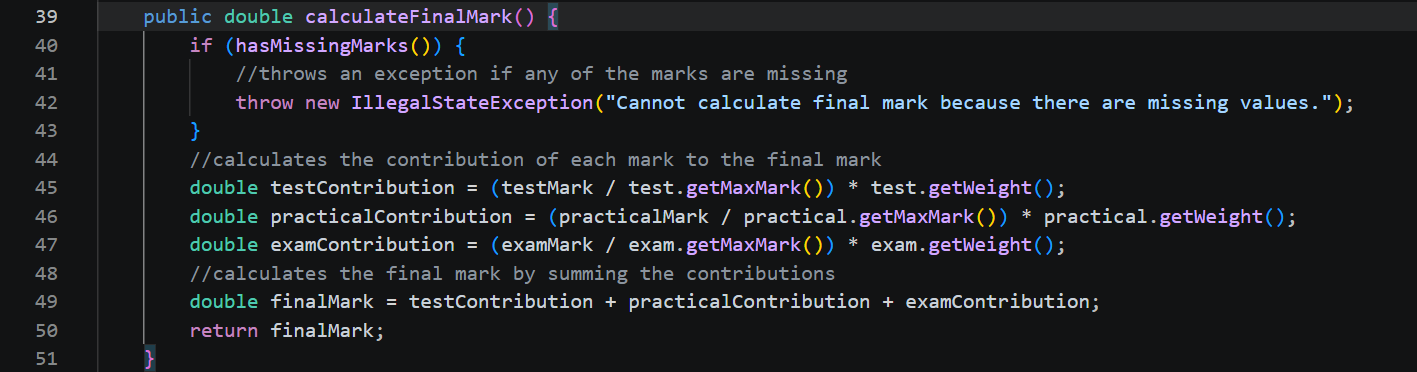
\includegraphics[width=0.92\textwidth]{Images/ch4_weighted_calculation.png}
\caption{Weighted contribution of each assessment in \texttt{IndividualMarksManager}.}
\label{fig:impl-code}
\end{figure}

\subsection{Persistence}
The \texttt{Database} class uses \texttt{java.nio.file} \cite{oracleFiles}. \texttt{saveData} builds a list of lines (a header followed by one line per student from the \texttt{StudentManager}), creates the parent folder with \texttt{Files.createDirectories} if needed, and writes the lines with \texttt{Files.write}. The course code is taken from the file name by removing the \texttt{marks.csv} suffix. Together with \texttt{loadData}, which skips blank, comment and header lines before building one \texttt{Student} per record, this provides create, read, update and delete behaviour on a plain text file. Output lines follow a fixed layout of student ID, name, assessment marks, final mark, grade and status.

Two design points are worth recording. First, \texttt{exportCSV} takes the destination \texttt{Path} as a parameter instead of prompting on the console, so any interface can call it. Second, \texttt{saveData} replaces the whole file, so saving without loading first would overwrite existing data. Course data is therefore loaded when a course is selected, before any edit is saved. The unused \texttt{importCSV} method was deleted once \texttt{importMarks} in \texttt{Lecturer} covered the same work, rather than keeping two import routes.

\subsection{Role layer and session handling}
Each role method exists in two forms. The parameterless form follows the Check-in 1 UML. The form that takes parameters and returns a \texttt{String} is what the interface calls, for example \texttt{viewClassSummary(course)} for the Head of Department. Both forms delegate to \texttt{CollectiveMarksManager} for statistics, so the maths is written once. \texttt{CourseSessionCoordinator} hands the interface the \texttt{StudentManager} and \texttt{Database} of the selected course.

\section{Advanced Features}\label{sec:adv}

\textbf{Graphical interface.} The Swing interface (\texttt{GUI}) offers a login screen, a lecturer screen and a Head of Department dashboard in one window. The lecturer table uses a non-editable \texttt{DefaultTableModel} and a custom cell renderer that shades incomplete rows red, while a Status column names the missing assessments. The Head of Department screen uses a split pane: choosing a course in the list updates the report beside it.

\textbf{Role-based access.} The login choice creates a \texttt{Lecturer} or a \texttt{HeadOfDepartment}. Only the lecturer object carries editing permission and offers the capture, update and import operations, so the read-only restriction is enforced by the objects and not only by hiding buttons.

\textbf{Multi-course management.} Each course has its own file, \texttt{<CODE>\_marks.csv}. A Head of Department can create a course, which also creates its file, or remove one after a confirmation dialog. Duplicate course codes are refused case-insensitively and blank fields are rejected.

\textbf{Flexible CSV import and export.} Import matches columns by header name rather than by position, trims the file path, and rejects files with missing headers with a readable message. Export asks for a destination with a file chooser and adds the \texttt{.csv} extension if it is missing.

\textbf{Analytics.} Class summaries, pass and fail counts, grade distribution, rankings and missing-mark lists are produced by \texttt{CollectiveMarksManager}, which ignores incomplete records so that missing data cannot distort averages. The all-course matrix gives the Head of Department a one-screen comparison across courses.

\textbf{Error handling.} Invalid marks, blank fields, unknown student numbers, malformed files and missing selections each produce a specific message and leave stored data unchanged.

\section{Testing Strategy}\label{sec:testing}

\subsection{Approach}
Testing was done in four layers. \emph{Component tests} exercised \texttt{Course}, \texttt{AssessmentComponent} and \texttt{IndividualMarksManager} from a console demonstration program. \emph{Integration tests} combined the domain classes with \texttt{Database} and the role classes. \emph{System tests} drove the Swing interface by hand with normal, boundary and invalid input. \emph{Regression checks} were repeated after each refactor (the \texttt{Module} to \texttt{Course} rename, the normalisation fix and the move from the console to the GUI). Expected results were worked out by hand before running each case, using the default weights of 30, 30 and 40.

\subsection{Test cases}
\begin{table}[htbp]
\centering
\small
\renewcommand{\arraystretch}{1.1}
\caption{Selected test cases with inputs and expected results.}
\label{tab:tests}
\begin{tabularx}{\textwidth}{@{}l >{\raggedright\arraybackslash}p{3.7cm} >{\raggedright\arraybackslash}p{3.3cm} X@{}}
\toprule
\textbf{ID} & \textbf{Scenario} & \textbf{Input} & \textbf{Expected result}\\
\midrule
T1 & Complete record & 60, 70, 80 & Final mark $18+21+32 = 71.0$; statistics calculated.\\
T2 & Update a mark & Exam 80 changed to 90 & Final mark recalculated to $75.0$.\\
T3 & Missing mark & Exam left blank & Row flagged, final mark withheld, status names the exam.\\
T4 & Boundary marks & 0 and 100 & Accepted and calculated correctly.\\
T5 & Out-of-range mark & 105 or $-5$ & \texttt{IllegalArgumentException}; error dialog; nothing saved.\\
T6 & Non-numeric mark & \texttt{abc} & Error dialog; record unchanged.\\
T7 & Blank or duplicate course code & Empty field, existing code & Rejected with a message; no file created.\\
T8 & No row selected & Press Update & Warning asking for a selection.\\
T9 & Unknown student number & Search for an absent ID & Message that no record was found.\\
T10 & Import with missing header & File without a required column & Rejected with a readable error; table unchanged.\\
T11 & Name containing a comma & \texttt{Surname, Name} & Saved quoted and loaded back as one field.\\
T12 & Export without extension & Name \texttt{results} & File written as \texttt{results.csv}.\\
\bottomrule
\end{tabularx}
\end{table}

All cases behaved as listed. The full run, including the interface cases, is shown in the demonstration recording submitted with this report.

\subsection{Evidence}
Figure~\ref{fig:evidence} shows console evidence for the component tests T1 to T3.

\begin{figure}[htbp]
\centering
\begin{subfigure}[t]{0.29\textwidth}\centering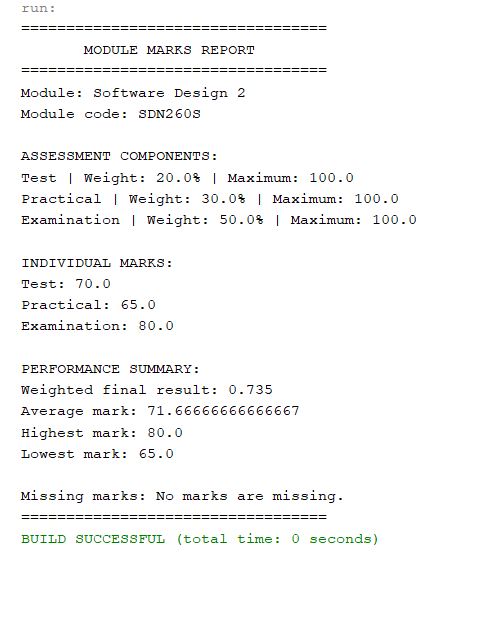
\includegraphics[height=4.3cm]{Images/ch4_complete_marks_test.png}\caption{T1: complete.}\end{subfigure}\hfill
\begin{subfigure}[t]{0.29\textwidth}\centering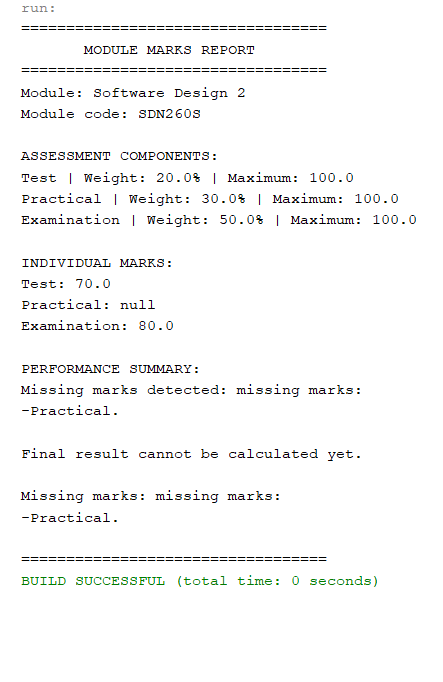
\includegraphics[height=4.3cm]{Images/ch4_missing_mark_test.png}\caption{T3: missing.}\end{subfigure}\hfill
\begin{subfigure}[t]{0.29\textwidth}\centering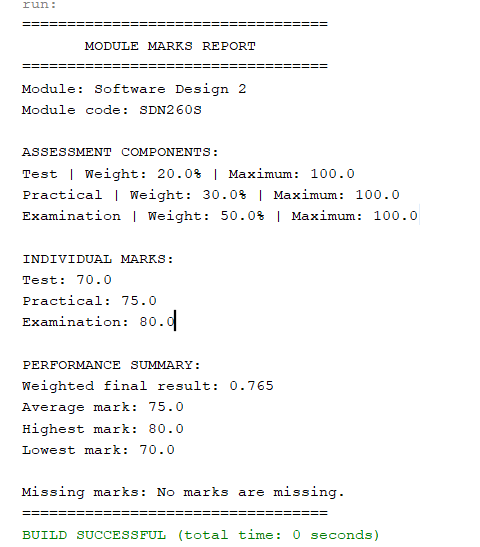
\includegraphics[height=4.3cm]{Images/ch4_updated_mark_test.png}\caption{T2: updated.}\end{subfigure}
\caption{Console output for the component tests.}
\label{fig:evidence}
\end{figure}

\subsection{Defects found}
Testing and review exposed four issues. (1) The demonstration program crashed when it asked for a result on an incomplete record, because it did not check \texttt{hasMissingMarks()} before calling the calculation; the check was added. (2) Final marks were wrong when assessments had different maximum marks, which led to the normalisation fix. (3) Inconsistent test CSV files caused null pointer errors on import, so validation and clear error prompts were added before records are read. (4) Review of \texttt{saveData} showed that it replaces the whole file, so data would be lost if a course were saved before it was loaded; course data is therefore loaded when a course is selected. A check before overwriting an exported file is still open (Section~\ref{sec:concl}).

\section{Reflections on GA2 and GA7}\label{sec:reflect}

\subsection{\gaTwoName}
Building the system meant applying what we had learned in programming and software design to a concrete problem. We used object-oriented decomposition to give every class a single responsibility, inheritance and abstraction to separate lecturer and Head of Department behaviour, and encapsulation to protect assessment weights. We reasoned numerically about the weighted mark and showed that scaling by the maximum mark is required, and we analysed the cost of each operation to justify choosing simple lists and linear passes over more complex structures. Working with \texttt{java.nio} and CSV forced us to deal with real data problems such as commas inside names, missing values and files whose columns are in a different order.

The most useful lesson was that applying knowledge is not the same as trusting it. The first version of the final-mark calculation looked correct and compiled, but it was wrong whenever assessments had different maximum marks. We only found it by comparing program output with hand-calculated values. After that we wrote the expected result before running each test, and we recorded our reasoning in the design decisions in Section~\ref{sec:decisions} so that it could be challenged.

\subsection{\gaSevenName}
Marks decide whether students progress, so an error in this software has consequences for people. We treated correctness as an ethical requirement as well as a technical one. The system refuses to calculate a final mark from incomplete data, rejects marks outside the valid range, and keeps missing marks out of class averages. Role-based access means the Head of Department can inspect results but cannot change them, which limits accidental or unauthorised edits.

Marks are also personal information, and in South Africa their handling falls under the Protection of Personal Information Act. In its current form the prototype stores plain-text CSV files with no authentication or encryption, and it keeps no audit trail of who changed a mark. Those are real limits, which is why the password feature is on its own branch for review and why we do not claim the system is ready for production use. On the positive side, the application needs only a standard Java installation and no server, the red highlighting and specific error messages make mistakes visible to non-technical users, and the modular design with explained code should keep long-term maintenance costs low.

\section{Team Collaboration Process}\label{sec:team}

\subsection{Organisation}
The eight-member group divided the work along the class boundaries agreed in the Check-in 1 UML diagram, so each member could develop and test a part independently. Table~\ref{tab:team} shows the areas of responsibility.

\begin{table}[htbp]
\centering
\small
\renewcommand{\arraystretch}{1.1}
\caption{Areas of responsibility.}
\label{tab:team}
\begin{tabularx}{\textwidth}{@{}>{\raggedright\arraybackslash}p{5.9cm} X@{}}
\toprule
\textbf{Area and classes} & \textbf{Member(s)}\\
\midrule
Marks management: \texttt{Course}, \texttt{AssessmentComponent}, \texttt{IndividualMarksManager} & \todo{names}\\
Students and analytics: \texttt{Student}, \texttt{StudentManager}, \texttt{CollectiveMarksManager} & \todo{names}\\
Roles: \texttt{User}, \texttt{Lecturer}, \texttt{HeadOfDepartment} & \todo{names}\\
Persistence and import/export: \texttt{Database} & \todo{names}\\
Interface and integration: \texttt{GUI}, \texttt{CourseSessionCoordinator}, \texttt{Main} & \todo{names}\\
Testing, documentation and demonstration & \todo{names}\\
\bottomrule
\end{tabularx}
\end{table}

\subsection{Version control and integration}
The project is kept in a shared GitHub repository whose \texttt{main} branch holds the working build \cite{gitdocs}. Work that was not ready, such as the password feature, was developed on a separate branch created from \texttt{main} so that a pull request can be reviewed before the change is merged. Commit messages describe what changed, for example the shared commit that updated \texttt{exportCSV} and \texttt{saveData} in \texttt{Database.java} and the classes that call them. Since Check-in 2 the original authors of \texttt{User}, \texttt{Lecturer}, \texttt{HeadOfDepartment} and \texttt{CollectiveMarksManager} made no further changes to them; the only later change came from that shared commit.
We had weekly group meetings on Microsoft Teams to check project status and discuss on progress. 

\subsection{Problems and lessons}
The main integration problems were inconsistent terminology (\texttt{Module} against \texttt{Course}), a duplicated import method, and a console-based design that did not suit a graphical interface. They were solved by agreeing on common names, deleting \texttt{importCSV} in favour of \texttt{importMarks}, and adding the text-returning method versions. The lessons were to agree interfaces before coding, to merge through review and not by direct edits, and to test the combined program early, because most defects appeared where one member's class met another's.

\section{Conclusion}\label{sec:concl}

The Marks Administration System meets its objectives: lecturers can capture, import and export marks with automatic weighted calculation, missing marks are flagged and kept out of statistics, and a Head of Department has read-only access to course summaries and rankings across several courses. The layered design allowed the interface to change from the console to Swing without rewriting the domain classes, and testing with normal and edge inputs exposed defects that were fixed before submission.

\textbf{Limitations and future work.} Password protection needs to be reviewed and merged into \texttt{main}. Data are stored unencrypted, no log or audit trail records changes, and exporting does not yet check for an existing file of the same name. The year-course functions are placeholders. A future version could move to a database, add file logging and extend the access model.


% -------------------------------
% REFERENCES AND APPENDIX
% -------------------------------
\clearpage
\printbibliography[heading=bibintoc, title={References}]

\appendix
\section{GitHub Repository}
The complete project (Java source code, NetBeans project files, sample CSV data, README and this report) is available at:\\
\githubLink


\end{document}
